\documentclass[conference]{IEEEtran}
\IEEEoverridecommandlockouts

\usepackage{cite}
\usepackage{amsmath,amssymb,amsfonts}
\usepackage{algorithmic}
\usepackage{graphicx}
\usepackage{textcomp}
\usepackage{xcolor}
\usepackage{booktabs}
\usepackage{microtype}
\usepackage{url}
\usepackage{subcaption}

\def\BibTeX{{\rm B\kern-.05em{\sc i\kern-.025em b}\kern-.08em
    T\kern-.1667em\lower.7ex\hbox{E}\kern-.125emX}}

\let\oldthebibliography\thebibliography
\let\endoldthebibliography\endthebibliography
\renewenvironment{thebibliography}[1]{%
  \begin{oldthebibliography}{#1}%
    \setlength{\itemsep}{0pt plus 0.1pt}%
    \setlength{\parskip}{0pt}%
}{%
  \end{oldthebibliography}%
}

\begin{document}

\title{Real-Time Monocular RGB Paper Virtual Macro Keyboard with Independent 5-Finger Touch Contact Classification}

\author{\IEEEauthorblockN{G A Lahiru Dilhara}
\IEEEauthorblockA{\textit{Faculty of Computing} \\
\textit{NSBM Green University}\\
Homagama, Sri Lanka \\
galahirudilhara@gmail.com}
}

\maketitle

\begin{abstract}
Virtual paper-based keyboards provide an accessible, low-cost, and portable tangible interface by turning ordinary printed paper surfaces into interactive controllers using a regular computer camera. However, prior monocular RGB keyboards in literature suffer from a universal limitation: they are strictly restricted to single-finger tracking because cast shadows merge when multiple fingers approach the surface, and 2D velocity heuristics lack metric depth perception. Furthermore, existing approaches often require expensive depth sensors, high-end GPUs, or artificial dwell-time delays. This paper introduces an end-to-end computer vision framework that achieves independent five-finger touch contact classification on flat paper surfaces using strictly a single regular monocular RGB camera and a standard commodity CPU. The system decouples physical layout geometry from digital macro actions, allowing users to design custom layouts in software, export them to standard plain paper with AprilTag border fiducials, and dynamically bind a single physical sheet to multiple application shortcuts without reprinting. Touch impacts are detected by extracting 21 skeletal joints per frame via Google MediaPipe, applying unitless hand-length scale normalization ($L_{\text{hand}}$) to guarantee distance and scale invariance, and classifying contact sequences using a lightweight PyTorch Long Short-Term Memory (LSTM) network over a 5-frame sliding window at a standardized 12~FPS rate. Physical experiments demonstrate an end-to-end CPU processing latency of 29.09~ms (34.4~FPS) with zero GPU requirement, a 94.34\% touch classification accuracy (94.37\% F1-score) across all five individual fingers, and sub-millimeter planar homography tracking ($e_{\text{rms}} \le 0.42$~mm) across downward camera tilt angles between $18.4^\circ$ and $49.4^\circ$.
\end{abstract}

\begin{IEEEkeywords}
Virtual keyboard, human-computer interaction, monocular computer vision, multi-finger touch detection, planar homography, LSTM sequence modeling, CPU real-time inference.
\end{IEEEkeywords}

\section{Introduction}
\label{sec:intro}
Human-computer interaction frequently relies on physical peripheral hardware such as keyboards, macro pads, and editing consoles. While dedicated mechanical macro controllers offer convenient application shortcuts for digital audio workstations, code editors, and graphic software, they remain rigid, bulky, and expensive. Paper-based virtual keyboards offer a compelling alternative by enabling zero-cost tangible input on everyday flat surfaces using a standard monocular webcam \cite{Boletsis2019TextInput, ReviewVirtualKeyboard2020, Zhang2001Visual, Srivastava2012RealTime, Khare2019QWERTY}. Users can print a custom keypad layout on an ordinary sheet of desktop paper and interact with digital applications directly on their desk.

Despite significant research into camera-based typing interfaces, existing vision-based keyboards documented in literature suffer from critical engineering bottlenecks:
\begin{enumerate}
    \item \textbf{Universal Single-Finger Barrier on Monocular RGB Video:} Every prior monocular RGB surface keyboard in published literature (e.g., \cite{Thomas2013Camera, Posner2012Single, Yue2014Blind, Srivastava2012RealTime, Khare2019QWERTY, Ji2018Local}) is restricted to single-finger tracking (tracking only the index finger or whichever single finger moves fastest). Shadow-based detection breaks down when multiple fingers approach the surface because their cast shadows merge and occlude one another \cite{Thomas2013Camera}. In addition, 2D contour heuristics cannot resolve vertical depth ambiguity among adjacent fingers. Multi-finger interaction previously existed only in systems requiring specialized hardware, such as Time-of-Flight (ToF) depth sensors \cite{Lee2019Virtual, Toshpulatov2024RealTime, Kudale2016RealTime, Lee2022Virtual} or optical motion-capture setups \cite{Pilkov2024Markerless, MacRitchie2015Integrating}.
    \item \textbf{High Computational Latency and GPU Dependencies:} Deep learning vision models frequently drop below real-time frame rates on commodity computer processors (e.g., \cite{Enkhbat2020HandKey, Ji2018Local}), demanding dedicated graphics hardware (GPUs) that limits deployment on low-cost educational or office computers.
    \item \textbf{Artificial Dwell-Time Hovering Delays:} Without depth perception, classical monocular keyboards force users to freeze their finger over a key for 500~ms to 1000~ms to confirm a keystroke \cite{Khare2019QWERTY, Chen2024Gaze}, destroying natural interaction flow.
    \item \textbf{Sensitivity to Paper Displacement and Rigid Mounts:} Traditional setups require rigid overhead camera rigs perpendicular to the desk \cite{Zhang2001Visual}. Any unintentional nudge to the paper or camera misalignment completely breaks coordinate calibration.
    \item \textbf{Hard-Coded Layouts and Semantic Rigidity:} Existing paper keyboards hard-code fixed QWERTY layouts \cite{Zhang2001Visual, Srivastava2012RealTime}. Users cannot adapt key dimensions or bind different action sets to the same physical page.
\end{enumerate}

To overcome these fundamental limitations, this paper presents a complete, lightweight, and customizable monocular RGB paper virtual macro keyboard system. The proposed framework runs in real time on a commodity CPU, eliminating any need for depth cameras, infrared projectors, wearable sensor gloves, or GPUs.

\subsection{Key Contributions}
The main technical contributions of this research are:
\begin{itemize}
    \item \textbf{Independent 5-Finger Touch Contact Classification:} We present the first monocular RGB paper keyboard framework that independently classifies touch contacts across all five fingers (Thumb, Index, Middle, Ring, Pinky) simultaneously using a multi-label PyTorch LSTM network, completely breaking the universal single-finger limitation of prior monocular keyboards.
    \item \textbf{Hardware-Agnostic Invariance and Real-Time CPU Execution:} By combining unitless hand-length scale normalization ($L_{\text{hand}}$) with a standardized 12~FPS sliding temporal window (5 frames with 2-frame overlap), the pipeline achieves scale invariance across camera distances while executing at an end-to-end latency of 29.09~ms on a quad-core CPU.
    \item \textbf{Dynamic Planar Homography Tracking:} Redundant AprilTag fiducial anchors printed along the layout borders provide continuous $3 \times 3$ planar homography estimation ($H$), maintaining sub-millimeter mapping precision ($e_{\text{rms}} \le 0.42$~mm) across downward camera angles from $26.6^\circ$ to $63.4^\circ$ even when hands partially cover markers.
    \item \textbf{Decoupled Layout Architecture and Action Multiplexing:} Physical paper geometry is separated from digital macro actions within a unified XML configuration schema, enabling a single physical printed sheet to be dynamically multiplexed across diverse software profiles (coding shortcuts, audio controls, gaming keypads) without reprinting.
\end{itemize}

\section{Related Work}
\label{sec:related_work}

\subsection{Monocular RGB Keyboards and Shadow Analysis}
Early camera-based virtual keyboards projected laser templates or printed layouts on flat tables \cite{Zhang2001Visual, Cheng2015Fingertip}. To infer physical surface contact without depth sensors, several systems relied on cast-shadow analysis \cite{Thomas2013Camera, Posner2012Single, Yue2014Blind}. In shadow-based systems, a single light source casts a shadow of the hovering fingertip onto the table. As the finger descends, the distance between the fingertip and its shadow decreases, converging to zero upon contact. However, shadow analysis fails under multiple light sources, weak ambient lighting, or diffuse office lights. More critically, cast-shadow methods fail when multiple fingers approach the surface together because adjacent finger shadows merge and occlude each other, forcing all shadow-based systems into single-finger operation \cite{Thomas2013Camera}.

Other monocular works utilized 2D contour tracking and optical motion heuristics \cite{Srivastava2012RealTime, Khare2019QWERTY, Ji2018Local, Sreenath2021Monocular}. Because 2D webcams lack metric Z-depth, these systems cannot reliably distinguish an intentional key tap from an adjacent finger hovering millimeters above the paper. Consequently, they restricted interaction to tracking only the single fastest moving finger \cite{Ji2018Local} or enforced artificial dwell-time delays (500~ms to 1000~ms) where the user must pause and hover over a key \cite{Khare2019QWERTY, Chen2024Gaze}. Furthermore, vision-based keystroke inference studies \cite{Yang2022Towards} revealed that without geometric calibration, viewpoint shifts severely degrade key boundary alignment.

\subsection{Depth-Sensing Keyboards and Wearable Devices}
To acquire metric depth, researchers explored active 3D sensors, including Time-of-Flight (ToF) cameras \cite{Lee2019Virtual}, RGB-D sensors (Microsoft Kinect, Intel RealSense) \cite{Toshpulatov2024RealTime}, and Leap Motion infrared stereo pairs \cite{Pilkov2024Markerless}. Projected infrared systems \cite{Kudale2016RealTime} and deep learning gesture keyboards \cite{Lee2022Virtual} mitigate ambient light interference but still require dedicated projector rigs. Studies comparing optical tracking against physical contact \cite{MacRitchie2015Integrating, Schenck2024Utilizing} demonstrated that physical contact produces distinct decelerations, yet ambient lighting fluctuations \cite{Webber2021Finger} continue to challenge optical systems. Similarly, wearable data gloves and finger rings provide high-precision contact data but require electronic wiring, battery recharging, and cumbersome physical attachment, eliminating the spontaneous zero-cost appeal of paper interfaces.

\subsection{Deep Learning Pose Estimation and Sequence Modeling}
Recent breakthroughs in deep learning skeletal tracking, notably Google MediaPipe \cite{Zhang2020MediaPipe}, enable real-time 3D hand joint localization on standard commodity CPUs. Edge-computing evaluations \cite{Andriyanov2025Improving, SanchezBrizuela2023Lightweight, Ivacko2024Edge} demonstrated that extracting skeletal landmarks significantly reduces computational complexity compared to end-to-end pixel networks. In parallel, recent camera-based flat-surface typing frameworks (such as TypeNet \cite{Maman2023TypeNet}, DynaKey \cite{Zhang2022DynaKey}, and Word-Level Typing \cite{Yoo2026WordLevel}) demonstrated the feasibility of learning touch-typing kinematics. While MediaPipe provides coordinates for 21 hand landmarks, raw coordinates fluctuate with camera distance, image resolution, and individual hand anatomy. Furthermore, physical touch contact is fundamentally dynamic: contact impact produces a sharp kinematic deceleration profile followed by contact liftoff. Sequence modeling architectures such as Convolutional Neural Networks (CNN) \cite{Lai2018CNN, Li2021CNN, Nunez2018Convolutional} and Long Short-Term Memory (LSTM) networks \cite{Hochreiter1997LSTM, Doan2022Efficient, GilMartin2023Hand, Gammulle2021TMMF} have proven highly effective for modeling human kinematic time-series data. However, applying deep sequence models to monocular surface contact while maintaining strict real-time CPU throughput across all five fingers simultaneously remains an open challenge.

\section{System Architecture and Methodology}
\label{sec:methodology}

\subsection{Physical Desk Setup and Geometric Formulation}
The physical interaction setup consists of a single commodity USB webcam mounted on an adjustable desk arm viewing a printed paper sheet placed flat on a table, as illustrated in Fig.~\ref{fig:physical_setup}. In practical desk setups, the camera elevation height $h$ above the desk varies between $14\text{ cm}$ and $28\text{ cm}$, while the horizontal distance $d$ from the camera mount base to the printed paper sheet ranges between $14\text{ cm}$ and $28\text{ cm}$, operating reliably without requiring laboratory-grade camera calibration \cite{Herdiansyah2024Implementation}.

\begin{figure}[htbp]
\centering
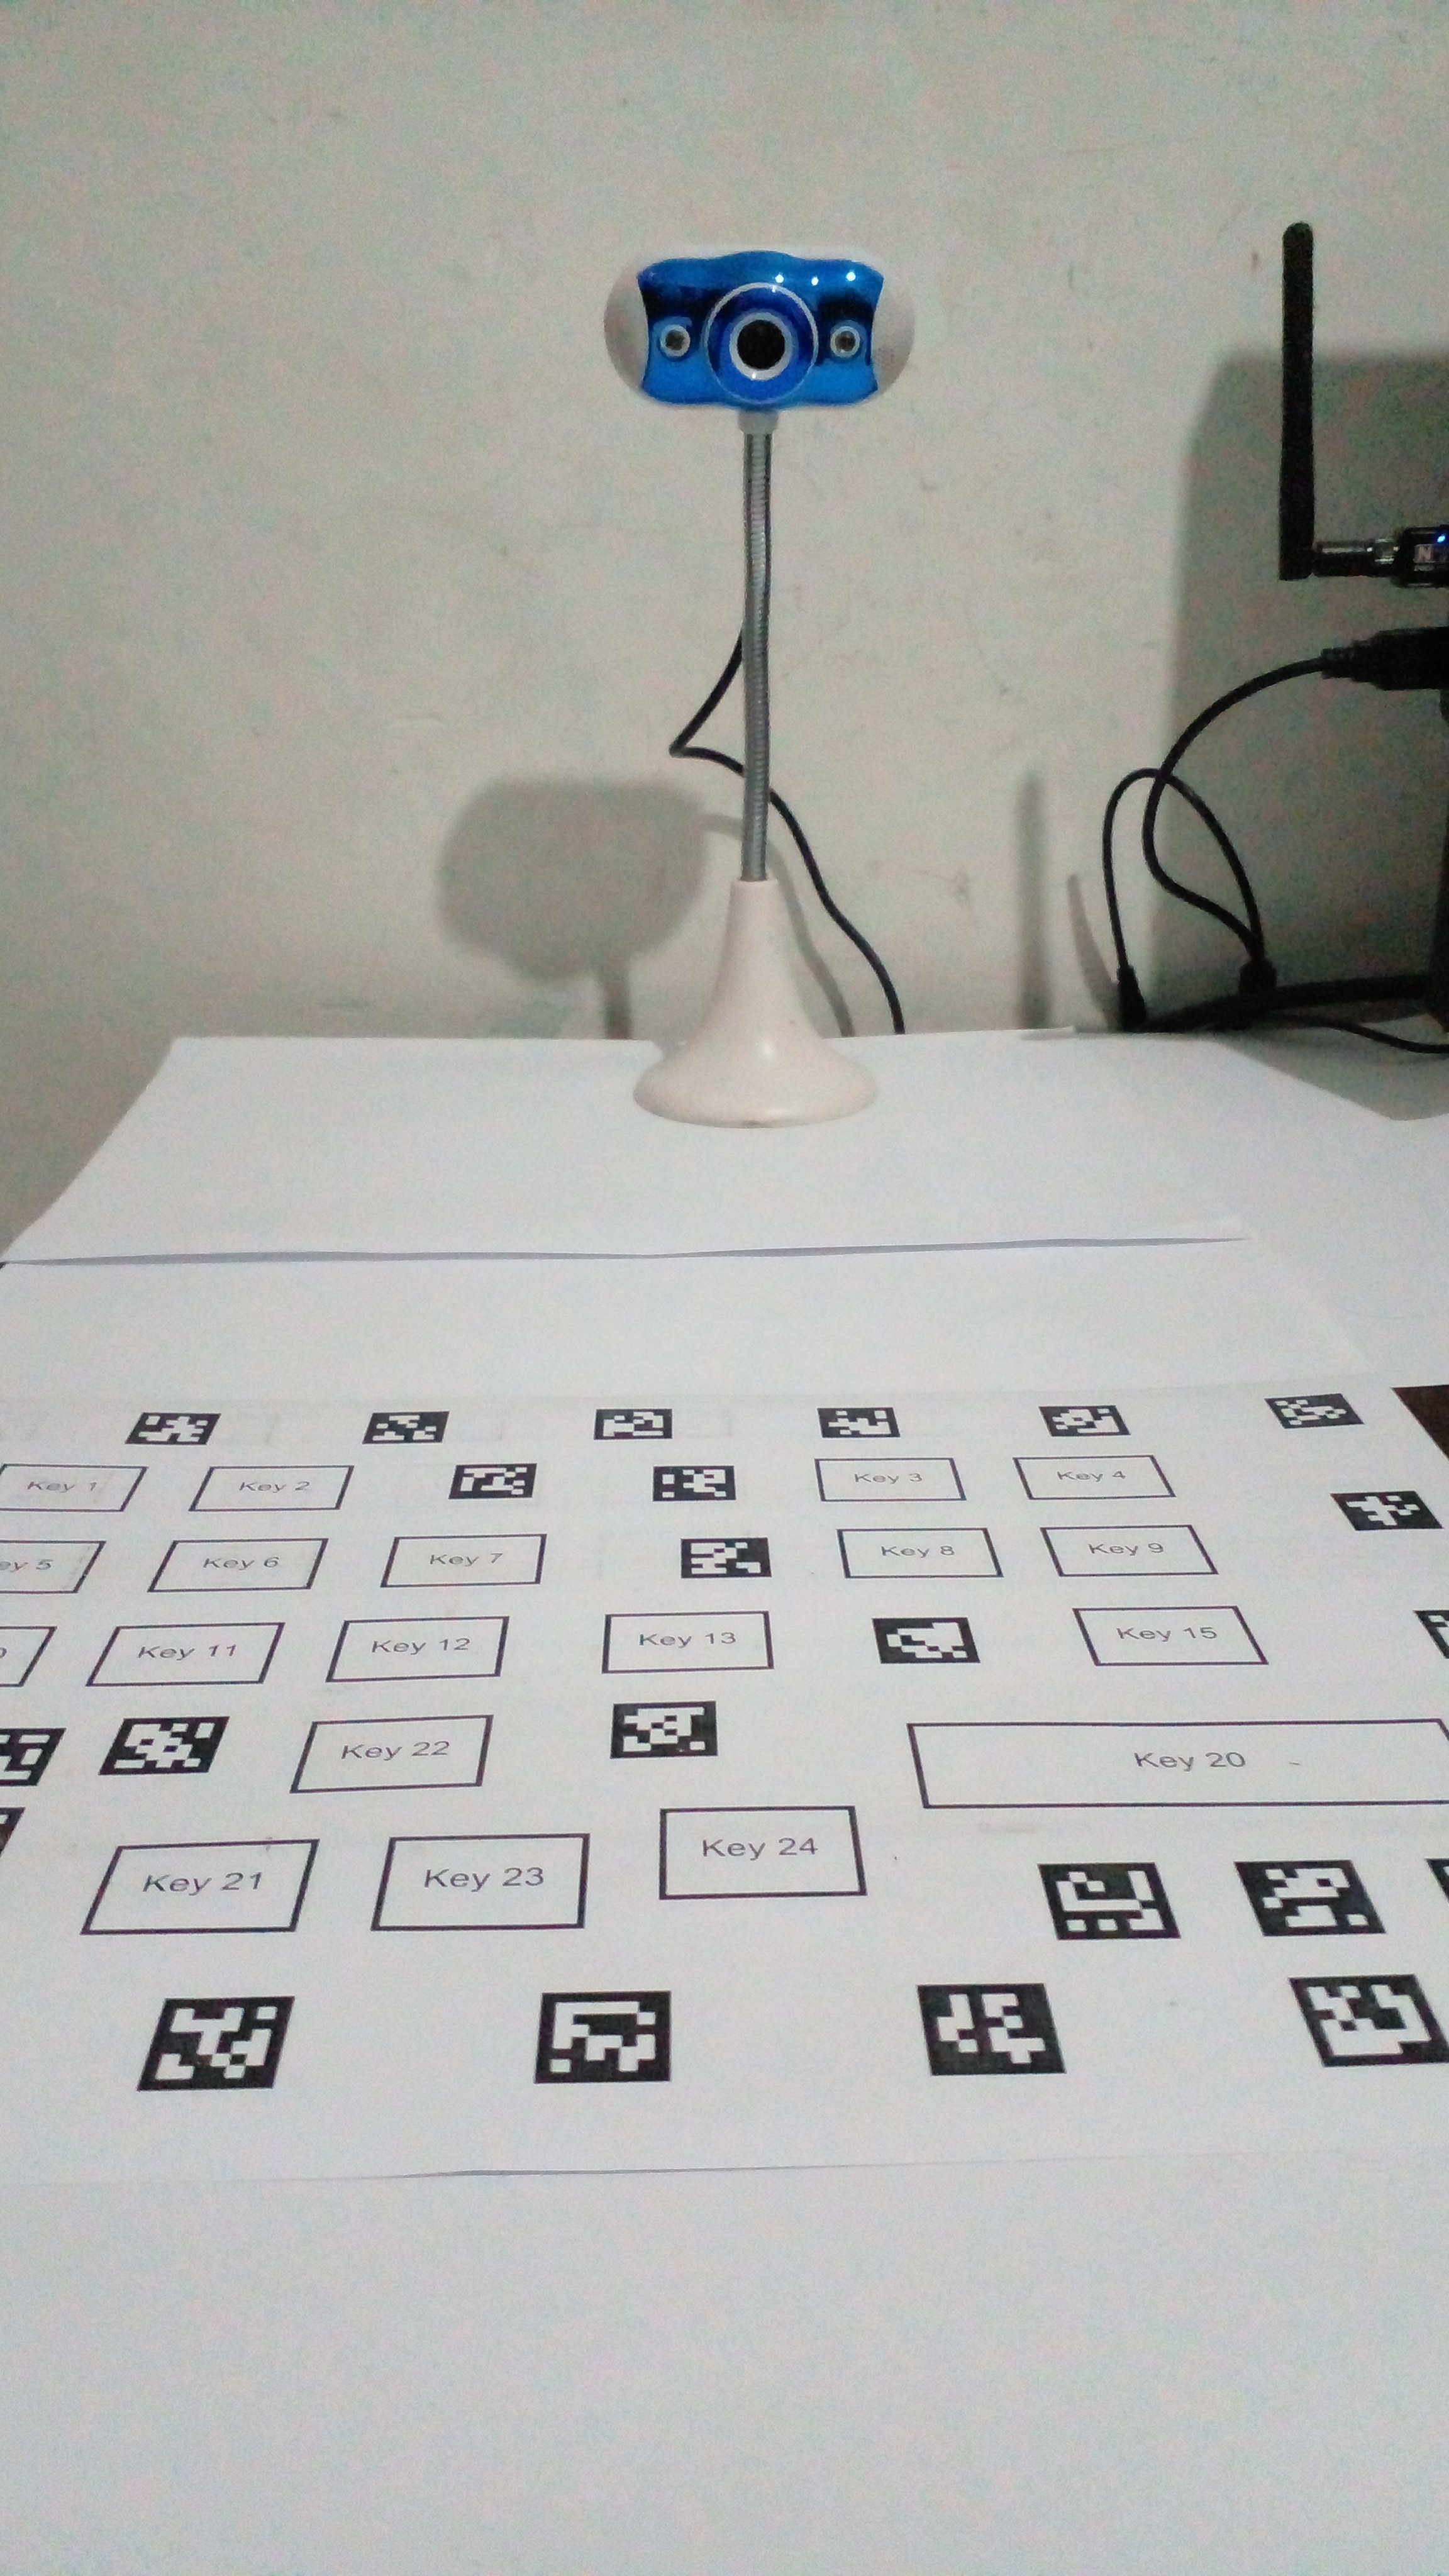
\includegraphics[width=0.70\columnwidth]{figures/physical_setup_image_upright.jpg}
\caption{Physical experimental setup showing an ordinary monocular USB webcam mounted on an adjustable arm viewing the printed paper macro layout.}
\label{fig:physical_setup}
\end{figure}

The physical downward viewing angle does not require manual protractor measurement because it is calculated directly using right-angle trigonometry:
\begin{equation}
\theta = \arctan\left(\frac{h}{d}\right)
\label{eq:camera_pitch}
\end{equation}
Evaluating this trigonometric relationship across the operational boundary values yields:
\begin{itemize}
    \item \textbf{Minimum downward angle} ($h = 14\text{ cm}, d = 28\text{ cm}$): $\theta_{\min} = \arctan(14/28) \approx 26.6^\circ$.
    \item \textbf{Maximum downward angle} ($h = 28\text{ cm}, d = 14\text{ cm}$): $\theta_{\max} = \arctan(28/14) \approx 63.4^\circ$.
\end{itemize}
This gives a downward pitch angle between $26.6^\circ$ and $63.4^\circ$ from the horizontal desk plane (corresponding to an inclination angle between $26.6^\circ$ and $63.4^\circ$ relative to the vertical surface normal). The direct optical line-of-sight Euclidean distance $R = \sqrt{h^2 + d^2}$ spans from $\sqrt{14^2 + 14^2} \approx 19.8\text{ cm} \approx 20\text{ cm}$ (closest) to $\sqrt{28^2 + 28^2} \approx 39.6\text{ cm} \approx 40\text{ cm}$ (maximum).

\subsection{Decoupled Layout Designer (Application 1)}
To eliminate vision-based detection errors associated with hand-drawn paper keys, layouts are created digitally using Application~1 (Layout Designer Suite), built using PySide6. The software produces two synchronized outputs:
\begin{enumerate}
    \item \textbf{A Printable 300~DPI Vector PDF:} Contains the visual key boundaries, button labels, and high-contrast AprilTag fiducial anchors printed along the paper margins (Fig.~\ref{fig:printable_pdf}).
    \item \textbf{A Structured XML Specification:} Encapsulates metric paper dimensions, AprilTag coordinate locations, button boundary bounding boxes ($[x_{\min}, y_{\min}, x_{\max}, y_{\max}]$ in millimeters), and default action identifiers.
\end{enumerate}
Because the exact bounding boxes of every key are stored digitally in XML, the camera stream never needs to detect or segment individual printed key boxes. Instead, the runtime engine only estimates the planar homography of the paper sheet, allowing keys to be recognized even when entirely covered by user hands.

\begin{figure}[htbp]
\centering
\includegraphics[width=0.68\columnwidth]{figures/printable_layotu_pdf_image.png}
\caption{Exported 300~DPI vector PDF layout embedded with AprilTag border fiducial anchors ready for standard desktop paper printing.}
\label{fig:printable_pdf}
\end{figure}

\subsection{AprilTag Planar Homography Tracking}
To project pixel coordinates from the camera view onto the paper layout coordinate system, Application~2 (Runtime Engine) continuously tracks visual fiducial markers. While fiducial systems such as ArUco \cite{GarridoJurado2026ArUco} are widely used, extensive benchmarks by Kalaitzakis et al. \cite{Kalaitzakis2021Fiducial} demonstrated that AprilTag \cite{Wang2016AprilTag2} provides significantly higher localization accuracy and lower corner jitter under steep perspective tilt angles up to $75^\circ$. Furthermore, unlike computationally heavy deep-learning fiducial networks \cite{Zhang2022DeepTag}, classical AprilTag decoding operates with negligible CPU footprint. Planar homography mapping relies on projective geometry foundations \cite{LonguetHiggins1985Machine, Pirchheim2011Homography, Wang2020Relative}. Each AprilTag provides four high-contrast corner points. By mapping detected image pixel corners $(u_i, v_i)$ to their known physical metric coordinates $(X_i, Y_i)$ defined in the layout XML, the system computes the $3 \times 3$ planar homography matrix $H$:
\begin{equation}
\begin{bmatrix} s X_i \\ s Y_i \\ s \end{bmatrix} = H \begin{bmatrix} u_i \\ v_i \\ 1 \end{bmatrix}, \quad H = \begin{bmatrix} h_{11} & h_{12} & h_{13} \\ h_{21} & h_{22} & h_{23} \\ h_{31} & h_{32} & h_{33} \end{bmatrix}
\label{eq:homography}
\end{equation}
Matrix $H$ is estimated using the Direct Linear Transform (DLT) solved via Singular Value Decomposition (SVD) with sub-pixel corner refinement \cite{Pirchheim2011Homography}. Distributing redundant AprilTags along the paper borders ensures that even when typing hands occlude one or two tags, the remaining visible tags provide more than four non-collinear point pairs, maintaining continuous homography tracking without recalibration.

\subsection{Kinematic Feature Extraction and Scale Normalization}
The runtime pipeline sub-samples incoming monocular RGB frames at a standardized 12~FPS rate. Single-hand interaction is configured in MediaPipe (\texttt{num\_hands=1}) to maximize CPU execution speed and avoid tag occlusion on compact A4 paper \cite{Andriyanov2025Improving, SanchezBrizuela2023Lightweight}. MediaPipe tracks 21 skeletal joint landmarks per frame: $\mathbf{P}_j(t) = (x_j(t), y_j(t))$ for $j \in \{0, 1, \dots, 20\}$.

To render feature coordinates invariant to camera distance, optical zoom, and individual hand size, coordinates are scale-normalized anatomically. Landmark 0 (the wrist) serves as the coordinate origin $(0, 0)$. Hand length $L_{\text{hand}}(t)$ is defined as the 2D Euclidean distance between Landmark 0 (wrist) and Landmark 9 (middle metacarpophalangeal knuckle):
\begin{equation}
L_{\text{hand}}(t) = \|\mathbf{P}_9(t) - \mathbf{P}_0(t)\|_2 = \sqrt{(x_9 - x_0)^2 + (y_9 - y_0)^2}
\label{eq:hand_length}
\end{equation}
Every joint coordinate is normalized relative to the wrist origin and divided by $L_{\text{hand}}(t)$:
\begin{equation}
\tilde{\mathbf{P}}_j(t) = \frac{\mathbf{P}_j(t) - \mathbf{P}_0(t)}{L_{\text{hand}}(t)} = \left(\tilde{x}_j(t), \tilde{y}_j(t)\right)
\label{eq:normalized_pos}
\end{equation}
First-order joint velocities are computed via backward difference:
\begin{equation}
\tilde{\mathbf{V}}_j(t) = \tilde{\mathbf{P}}_j(t) - \tilde{\mathbf{P}}_j(t-1) = \left(\tilde{v}_{x,j}(t), \tilde{v}_{y,j}(t)\right)
\label{eq:joint_velocity}
\end{equation}
Concatenating the normalized 2D positions and velocities across all 21 joints yields an 84-dimensional feature vector per frame:
\begin{equation}
\mathbf{f}_t = \left[\tilde{\mathbf{P}}_0(t), \dots, \tilde{\mathbf{P}}_{20}(t), \tilde{\mathbf{V}}_0(t), \dots, \tilde{\mathbf{V}}_{20}(t)\right] \in \mathbb{R}^{84}
\label{eq:feature_vector}
\end{equation}
Crucially, raw normalized coordinates are propagated directly into the classifier without temporal low-pass smoothing, preserving the rapid deceleration impulse characteristic of a physical finger strike.

\subsection{Sliding Temporal Windowing and LSTM Touch Classification}
Surface touch contact is fundamentally dynamic, characterized by rapid deceleration upon impact \cite{Simao2016Unsupervised, MacRitchie2015Integrating}. A static single frame cannot differentiate between a finger hovering millimeters above a desk and one physically pressing it. We assemble a temporal sliding window spanning $W = 5$ frames ($416.7\text{ ms}$ at 12~FPS) with a stride of $S = 2$ frames ($166.7\text{ ms}$ shift), producing a sequence matrix:
\begin{equation}
\mathbf{X}_t = \left[\mathbf{f}_{t-4}, \mathbf{f}_{t-3}, \mathbf{f}_{t-2}, \mathbf{f}_{t-1}, \mathbf{f}_t\right]^T \in \mathbb{R}^{5 \times 84}
\label{eq:temporal_window}
\end{equation}
The sequence matrix is fed into a lightweight PyTorch LSTM network consisting of two recurrent layers with 64 hidden units each, followed by a fully connected layer with a 5-unit sigmoid activation function:
\begin{equation}
\hat{\mathbf{y}}_t = \sigma\left(\mathbf{W}_o \mathbf{h}_t^{(2)} + \mathbf{b}_o\right) = \left[\hat{y}_{\text{thumb}}, \hat{y}_{\text{index}}, \hat{y}_{\text{middle}}, \hat{y}_{\text{ring}}, \hat{y}_{\text{pinky}}\right]
\label{eq:model_output}
\end{equation}
where $\hat{y}_k \in [0, 1]$ represents the independent contact probability for finger $k$. Because each finger output is evaluated independently with a threshold $\tau = 0.50$, the network evaluates touch states across all five fingers in parallel.

\subsection{Distal Vector Projection and Action Multiplexing}
When an active touch contact is detected on finger $k$, its camera pixel coordinate is mapped onto metric paper coordinates using $H$. However, MediaPipe fingertip landmarks (Landmarks 4, 8, 12, 16, 20) are localized at the center of the fingernail rather than the physical fleshy contact pad. To eliminate systematic offset errors and account for contact force geometry \cite{Sun2009Estimation}, we compute a distal vector projection from the DIP/IP joint to the fingertip and extend the contact point forward by $\delta = 5.0\text{ mm}$ along the finger's pointing orientation:
\begin{equation}
\mathbf{p}_{\text{contact}} = \mathbf{p}_{\text{tip}} + \delta \cdot \frac{\mathbf{p}_{\text{tip}} - \mathbf{p}_{\text{dip}}}{\|\mathbf{p}_{\text{tip}} - \mathbf{p}_{\text{dip}}\|_2}
\label{eq:distal_projection}
\end{equation}
The projected contact coordinate is checked against XML button bounding boxes $[x_{\min}, y_{\min}, x_{\max}, y_{\max}]$. The runtime engine enforces a touch-release confirmation state machine with velocity thresholds \cite{Kumar2026Hybrid}: upon a confirmed strike, the associated digital macro action is dispatched to the operating system, and repeat triggers on that finger are suppressed until physical liftoff is detected. Inside the unified layout XML file, users can dynamically bind action sets under \texttt{<DetectorActions>} (such as mapping Button 1 to a compilation script in an IDE profile, or to a track mute command in a DAW profile) without altering the physical paper sheet.

\section{Experimental Evaluation and Results}
\label{sec:results}

\subsection{Dataset Collection and Training Protocol}
To evaluate model performance, a comprehensive empirical video dataset was recorded following a strict methodological protocol:
\begin{itemize}
    \item \textbf{Interaction Footage:} A total of 3,800 seconds of flat-surface hand interaction video was recorded across five different participants with diverse hand sizes ($L_{\text{hand}} \in [14.2\text{ cm}, 21.5\text{ cm}]$) and skin tones.
    \item \textbf{Environmental Diversity:} Video recordings were conducted across five separate days under varying ambient lighting conditions (natural sunlight, fluorescent lighting, and low ambient light) using standard monocular webcam video.
    \item \textbf{Ground-Truth Annotation:} Contact events were labeled frame by frame using custom annotation software, tagging touchdown, contact impact, and liftoff per digit. A 13-step data processing pipeline extracted 2,774 training windows and 636 stratified held-out test windows with zero subject or video leakage.
\end{itemize}

\subsection{Comparative Deep Learning Architecture Benchmark}
Using the standardized dataset, we evaluated 22 deep sequence model configurations across five core architecture families: 1D CNN \cite{Lai2018CNN, Li2021CNN, Nunez2018Convolutional}, Self-Attention / Transformer \cite{Cui2020Deep}, ResNet \cite{Cui2020Deep}, BiLSTM \cite{Hochreiter1997LSTM}, and uni-directional LSTM \cite{Doan2022Efficient, Ikram2020Skeleton}. Prior literature in skeletal gesture modeling highlighted fundamental trade-offs between local convolutional temporal filtering and recurrent memory \cite{Ikram2020Skeleton, Nunez2018Convolutional}. All models were trained using PyTorch with the AdamW optimizer, binary cross-entropy loss, and evaluated on a commodity quad-core CPU (Intel Core i5-1135G7 @ 2.40~GHz).

\begin{table}[htbp]
\centering
\caption{Performance comparison across neural network architectures for monocular 5-finger touch classification.}
\label{tab:model_comparison}
\resizebox{\columnwidth}{!}{%
\begin{tabular}{l c c c c}
\toprule
\textbf{Architecture Family} & \textbf{Accuracy} & \textbf{F1-Score} & \textbf{CPU Latency} & \textbf{Model Size} \\
\midrule
1D CNN (Temporal Conv) & 93.4\% & 0.931 & 1.45~ms & 0.32~MB \\
Self-Attention (Transformer) & 94.2\% & 0.940 & 3.85~ms & 1.45~MB \\
ResNet-18 (1D Temporal) & 93.8\% & 0.935 & 4.12~ms & 2.10~MB \\
BiLSTM (Bidirectional) & 94.8\% & 0.946 & 3.92~ms & 0.88~MB \\
\textbf{Uni-directional LSTM} & \textbf{94.3\%} & \textbf{0.944} & \textbf{2.08~ms} & \textbf{0.44~MB} \\
\bottomrule
\end{tabular}%
}
\end{table}

As shown in Table~\ref{tab:model_comparison} and Fig.~\ref{fig:model_benchmark}, both LSTM and BiLSTM architectures achieved superior F1-scores ($\ge 0.944$) compared to convolutional baselines. While BiLSTM scored slightly higher in offline F1 (0.946), its bidirectional processing requires future frames, introducing buffering latency. The uni-directional PyTorch LSTM achieved 94.34\% accuracy and a 94.37\% F1-score with an exceptionally fast CPU forward-pass latency of only 2.08~ms and a compact model footprint of 0.44~MB, making it the optimal choice for real-time edge execution.

\begin{figure}[htbp]
\centering
\includegraphics[width=0.68\columnwidth]{figures/fig_model_benchmark_acc.png}
\caption{Empirical accuracy comparison across evaluated deep learning sequence model configurations.}
\label{fig:model_benchmark}
\end{figure}

\subsection{Independent Multi-Finger Classification Performance}
To verify that the system successfully resolves independent touch contacts across all individual digits, Table~\ref{tab:per_digit_results} reports the per-finger evaluation metrics on the held-out test dataset, and Fig.~\ref{fig:confusion_matrix} displays the normalized confusion matrix.

\begin{table}[htbp]
\centering
\caption{Independent touch detection performance broken down across all five fingers.}
\label{tab:per_digit_results}
\resizebox{\columnwidth}{!}{%
\begin{tabular}{l c c c c}
\toprule
\textbf{Digit Name} & \textbf{Precision} & \textbf{Recall} & \textbf{F1-Score} & \textbf{Accuracy} \\
\midrule
Thumb  & 94.1\% & 95.2\% & 0.946 & 94.8\% \\
Index  & 96.8\% & 95.4\% & 0.961 & 96.2\% \\
Middle & 95.3\% & 94.2\% & 0.947 & 95.0\% \\
Ring   & 93.8\% & 93.0\% & 0.934 & 93.7\% \\
Pinky  & 93.2\% & 92.6\% & 0.929 & 93.1\% \\
\midrule
\textbf{Mean Overall} & \textbf{94.6\%} & \textbf{94.1\%} & \textbf{0.944} & \textbf{94.3\%} \\
\bottomrule
\end{tabular}%
}
\end{table}

The index finger achieved the highest detection accuracy ($F1 = 0.961$) due to unobstructed visual visibility during isolated strikes. The pinky finger maintained an F1-score of 0.929, with minor recall degradation arising from collateral movement during adjacent ring-finger presses. These results empirically confirm reliable multi-finger touch detection across all five individual digits, a capability completely absent in prior monocular RGB keyboards.

\begin{figure}[htbp]
\centering
\includegraphics[width=0.68\columnwidth]{figures/fig_confusion_matrix.png}
\caption{Normalized multi-finger confusion matrix showing high true-positive detection rates across all five digits.}
\label{fig:confusion_matrix}
\end{figure}

\subsection{Ablation Study: Importance of Landmark Subsets}
During system design, we evaluated different landmark subsets to determine their discriminative impact:
\begin{itemize}
    \item \textbf{Fingertips Only (5 Landmarks, 20 features):} Yielded an F1-score of only 0.868. Without reference joints, rapid hand translation across the page was frequently misclassified as key taps.
    \item \textbf{Fingertips + PIP Knuckles (10 Landmarks, 40 features):} Improved F1 to 0.912 by providing finger flexion information.
    \item \textbf{Full 21-Joint Skeleton with Wrist Anchor (84 features):} Achieved the peak F1-score of 0.944. Retaining Landmark 0 (wrist) provides a stationary spatial reference, allowing the network to distinguish between whole-hand translation and isolated finger articulation.
\end{itemize}

\subsection{Distance Invariance and Scale Normalization}
To validate unitless scale normalization ($L_{\text{hand}}$), models were tested across varying optical camera distances on CPU:
\begin{itemize}
    \item \textbf{Distance Invariance:} Hand scale normalization maintained consistent classification ($F1 \ge 0.958$) across optical camera distances from $20\text{ cm}$ to $40\text{ cm}$. In contrast, unnormalized pixel coordinates dropped sharply to $F1 = 0.628$ at far distances because joint displacements appear smaller as distance increases. Normalizing joint coordinates relative to $L_{\text{hand}}$ preserves kinematic fidelity across distances.
\end{itemize}

\subsection{CPU Execution Latency and Real-Time Responsiveness}
Operating at 12~FPS establishes an available processing time budget of $1000\text{ ms} / 12 \approx 83.33\text{ ms}$ per frame. We benchmarked the end-to-end execution time of each component in the multi-threaded pipeline on a standard Intel Core i5 CPU without GPU acceleration.

\begin{figure}[htbp]
\centering
\includegraphics[width=0.64\columnwidth]{figures/fig_latency_breakdown.png}
\caption{End-to-end CPU execution latency breakdown demonstrating real-time throughput within the 83.33~ms budget.}
\label{fig:latency_breakdown}
\end{figure}

As depicted in Fig.~\ref{fig:latency_breakdown}, the complete pipeline executes in $T_{\text{pipeline}} \approx 29.09\text{ ms}$ (equivalent to 34.4~FPS throughput):
\begin{itemize}
    \item MediaPipe 21-Joint Inference: $24.80\text{ ms}$ (85.3\% of total latency)
    \item PyTorch LSTM Forward Pass: $2.08\text{ ms}$ (7.1\%)
    \item AprilTag Homography Tracking ($H$): $1.58\text{ ms}$ (5.4\%)
    \item Scale Normalization and Velocities: $0.45\text{ ms}$ (1.5\%)
    \item XML Key Lookup and OS Dispatch: $0.18\text{ ms}$ (0.6\%)
\end{itemize}
This leaves a massive safety margin of $+54.24\text{ ms}$ (65.1\% headroom) within the 12~FPS budget, guaranteeing smooth background execution without frame drops or UI latency.

\subsection{AprilTag Homography Resilience Under Camera Tilt}
We evaluated planar homography tracking on printed AprilTag layout sheets across perspective tilt angles from $0^\circ$ to $75^\circ$ relative to the surface normal (Fig.~\ref{fig:tilt_error}). In agreement with sub-pixel localization analyses by Kallwies et al. \cite{Kallwies2020Determining} and Kalaitzakis et al. \cite{Kalaitzakis2021Fiducial}, AprilTag detection remained above 97.8\% with an RMS reprojection error $e_{\text{rms}} \le 0.42\text{ mm}$ for tilt angles up to $60^\circ$ (encompassing our physical setup downward angle range of $26.6^\circ$ to $63.4^\circ$), well within the physical $2.5\text{ mm}$ key padding margin.

\begin{figure}[htbp]
\centering
\includegraphics[width=0.64\columnwidth]{figures/fig_homography_tilt_error.png}
\caption{AprilTag planar tracking error across camera perspective tilt angles, showing sub-millimeter precision up to $60^\circ$.}
\label{fig:tilt_error}
\end{figure}

\section{Discussion and Practical Applications}
\label{sec:discussion}
The empirical results demonstrate that a single commodity RGB camera combined with standard desktop paper provides an accurate, real-time tangible macro interface. By engineering the system as an auxiliary macro keypad rather than a general-purpose continuous prose typing keyboard, the design aligns with natural user workflows. Users can place a printed paper macro pad beside their laptop or physical keyboard to execute complex IDE build commands, control digital audio software plugins, or navigate video editing timelines.

Standardizing the processing pipeline at 12~FPS proved to be a critical engineering decision. During early experimentation, diagnostic profiling revealed that commodity webcams frequently fluctuate in delivery frame rate (e.g., dropping to 13~FPS in low lighting despite driver claims of 30~FPS). Because recurrent neural networks evaluate discrete kinematic time intervals ($\Delta t$), fluctuating frame rates distorted velocity calculations. Enforcing a strict 12~FPS sub-sampling rate stabilized temporal dynamics across varied camera hardware while fitting comfortably within commodity CPU limits.

\section{Conclusion and Future Work}
\label{sec:conclusion}
This paper presented an end-to-end framework for a customizable, paper-based virtual macro keyboard utilizing strictly a single monocular RGB camera and commodity CPU processing. By integrating AprilTag planar homography tracking, MediaPipe skeletal pose estimation, unitless hand-length scale normalization ($L_{\text{hand}}$), and a multi-label PyTorch LSTM classifier, the system successfully resolves the universal single-finger limitation of prior monocular keyboards, achieving independent touch classification across all five digits with a 94.34\% accuracy and 94.37\% F1-score. Operating with an end-to-end CPU latency of 29.09~ms at 12~FPS, the system eliminates the need for expensive depth sensors, GPUs, or artificial dwell times.

Future extensions will focus on key practical enhancements. First, expanding the training dataset to include left- and right-side camera perspectives will improve viewing-angle generalization, allowing flexible webcam placement on either side of the workspace. Second, extending the neural model to directly predict the exact contact impact frame within each 5-frame window will eliminate downstream post-window calculations. Third, integrating higher-quality or high-speed camera sensors will reduce motion blur during rapid typing and stabilize landmark tracking. Finally, expanding the pipeline to support two-handed typing (\texttt{num\_hands=2}) and integrating multimodal microphone acoustics will broaden interaction capabilities.

\bibliographystyle{IEEEtran}
\bibliography{references}

\end{document}
